\addtolength{\hoffset}{-2.25cm}
\addtolength{\textwidth}{4.5cm}
\addtolength{\voffset}{-2.5cm}
\addtolength{\textheight}{5cm}
\setlength{\parskip}{0pt}
\setlength{\parindent}{15pt}
\documentclass[10pt,a4paper]{letter}
\usepackage[utf8]{inputenc}
\usepackage{amsmath}
\usepackage{amsfonts}
\usepackage{amssymb}
\usepackage{graphicx}
\begin{document} 

To approximate the integral $\iint f(x,y) dA$ on the unit disk for a function\\ $f: \mathbb{R}^2 \to \mathbb{C}$, we derive a formula which can integrate a polynomial $p(x,y) \in \mathbb{P}_k$ exactly on this region.  The goal will be to obtain an approximation to the integral of the form
$$\iint_{S_2} f(x,y) dA \approx \sum_{i=1}^M f(x_i, y_i)$$ 
We first transform an integral of a monomial $\iint_{S_2} x^\alpha y^\beta dA$ so that it separates into the product of two single integrals.  This can be done with the choice of polar coordinates
$$x = r \cos(\theta), y = r \sin(\theta) \text{ with } -1 \leq r \leq 1,\ \  -\pi/2 \leq \theta \leq \pi/2.$$
The Jacobian of this transformation is $r$ so we obtain
\begin{align*}
\iint x^\alpha y^\beta dx dy &= \int_{-\pi/2}^{\pi/2} \int_{-1}^1 |r| r^{\alpha + \beta} \cos^\alpha \theta \sin^\beta \theta\ dr \ d\theta\\
 &= \left(\int_{-\pi/2}^{\pi/2} \cos^\alpha \theta \sin^\beta \theta \ d\theta\right)\left( \int_{-1}^1 |r| r^{\alpha + \beta} \ dr \right)
\end{align*}
We seek Gauss formuals for these single integrals.  We note that if $\alpha$ or $\beta$ is odd, the integral is zero.  Therefore the product formula must be exact for all polynomials in $\mathbb{P}_k$ and maintain this zero condition.\\

Consider formulas of the form
$$\int_{-\pi/2}^{\pi/2} P(\cos \theta, \sin \theta)\ d\theta \approx \sum_{i=1}^M A_i P(\cos \theta_i, \sin \theta_i)$$
$$ \text{ where } \theta_i = -\theta_{m-i+1}, A_i = A_{m-i+i}\ i = 1 \dots M$$
$$\int_{-1}^1 |r| f(r)\ dr \approx \sum_{i=1}^M B_i f(r_i),$$ $$\text{ where } r_i = -r_{M-i+1} B_i=B_{M-i+1}, i=1,\dots,M$$
Where the first formula is exact when $P(\cos\theta, \sin\theta)$ is a linear combination of terms $(\cos \theta)^{2q}(\sin\theta)^r, 2q+r \leq k, q, r \geq 0$ and the second formula is exact when $f(r) \in \mathbb{P}_k.$\\

Theorem (Stroud) If the formulas above satisfy the specified conditions, their product is exact in $\mathbb{P}_k.$\\

Since $|r|$ does not change sign on $[-1,1]$, a Gauss formula for the second equation can be constructed by the standard methods.  The first formula can be put into a more standard form. Let
\begin{align*}
s&=\sin\theta, \ 1-s^2 = \cos^2 \theta\\
ds &= \cos\theta, \ d\theta = (1-s^2)^{-1/2}\ ds
\end{align*}
It is straightforward to show that if the formula
$$\int_{-1}^1 (1-s^2)^{-1/2} f(s) ds \approx \sum_{i=1}^M A_i f(s_i),$$ $$s_i = -s_{M-i+1}, A_i = A_{M-i+1}, i=1, \dots, M$$
is exact for all polynomials $f(s)$ in $\mathbb{P}_k$ then transforming in this way gives a formula satisfying the desired condition.  It is a Gauss-Chebyshev formula of the first kind.  The points and coefficients in this formula are known in closed form.
$$s_i = \cos\left(\frac{(2i-1)\pi}{2M}\right), A_i = \pi/M, i = 1, \dots, M$$\\

The quadrature points are shown below for $M = 1 \dots 4$\\

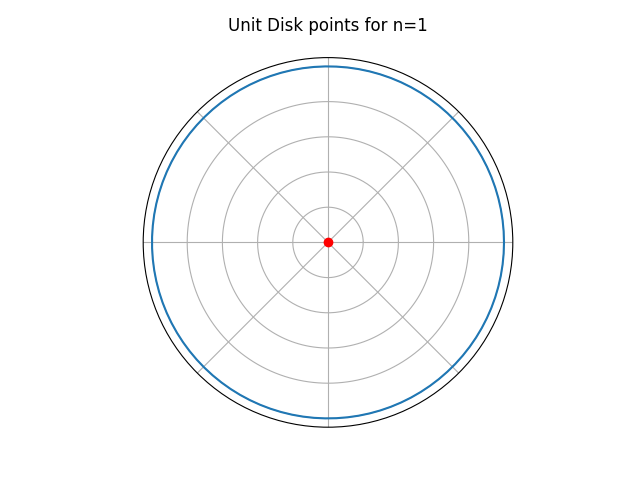
\includegraphics[scale=.5]{disk0_n1}
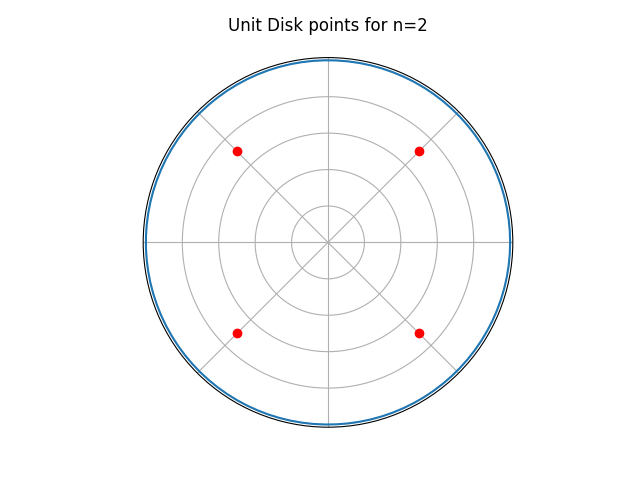
\includegraphics[scale=.5]{disk0_n2}
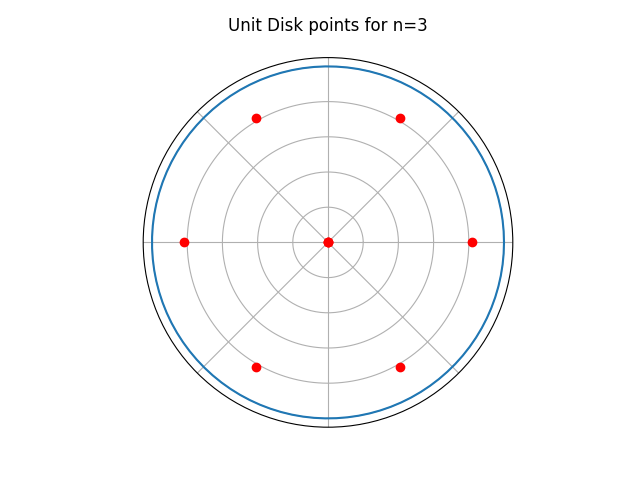
\includegraphics[scale=.5]{disk0_n3}
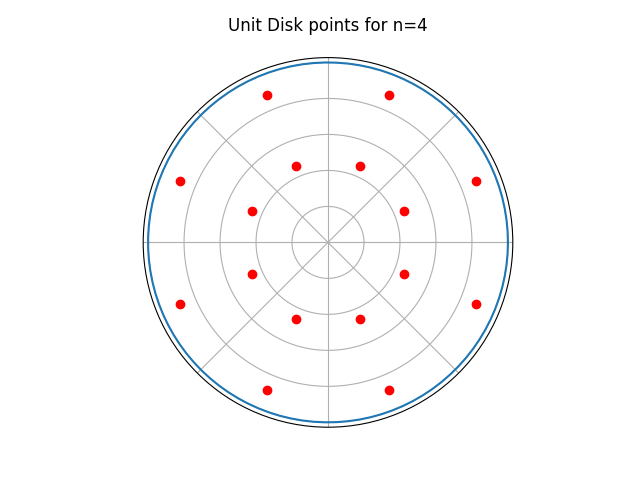
\includegraphics[scale=.5]{disk0_n4}

\pagebreak
It would be desirable to construct an integration formula for an annulus since this will allow integration over the annular cladding region and should be able to provide an alternative quadrature for a disk, which may place a heavier weight on points near the center of the disk.
To construct an integration formula for an annular region given by $$r1 < r < r2,\ \  -\pi \leq \theta \leq 3\pi/2,$$ we begin by writing the integral as a sum of integrals
\begin{align*}
\int_{-\pi/2}^{3\pi/2} \int_{r_1}^{r_2} r f(r,\theta)\ dr d\theta &= \int_{-\pi/2}^{\pi/2} \int_{r_1}^{r_2} r f(r,\theta)\ dr d\theta + \int_{\pi/2}^{3\pi/2} \int_{r_1}^{r_2} r f(r,\theta)\ dr d\theta\\
&= \int_{-\pi/2}^{\pi/2} \int_{r_1}^{r_2} r f(r,\theta)\ dr d\theta + \int_{-\pi/2}^{\pi/2} \int_{r_1}^{r_2} r f(r,\theta')\ dr d\theta'
\end{align*}
where $\theta' = \theta - \pi$ so $\theta = \theta'+\pi$ and $\sin\theta' = -\sin\theta, \cos\theta' = -\sin\theta$.  Next, let $\bar{r} = \frac{r_2+r_1}{2}, \gamma = \frac{r_2-r_1}{2}$ and $c = \frac{\bar{r}}{\gamma} \geq 1$ and consider the change of variables$$r = \gamma \rho + \bar{r} = \gamma(\rho + c),\ dr = \gamma\ d\rho$$
Then the integral for the annulus above may be written as 
$$\gamma^2\left(\int_{-\pi}^{\pi/2}\int_{-1}^1 (\rho + c) f(\gamma(\rho + c), \theta) \ d\rho d\theta +
\int_{-\pi}^{\pi/2}\int_{-1}^1 (\rho + c) f(\gamma(\rho + c), \theta') \ d\rho d\theta'\right)$$
We see that, as in the case of the disk discussed earlier, the term $\rho + c$ does not change sign on the interval $[-1,1]$ and the limits of integration are amenable to the Gauss-Chebyshev method used for the disk so in this case also, a Gauss formula should be constructable by standard methods.\\

With this formulation we obtain the following disk quadrature points as shown below, but the computed weights must be multiplied by a factor of $2c$ for reasons which are not currently understood.  This method requires $2n^2$ function evaluations (twice as many as for the other quadrature) to be exact for polynomials of degree $k \leq 2n-1$ \\

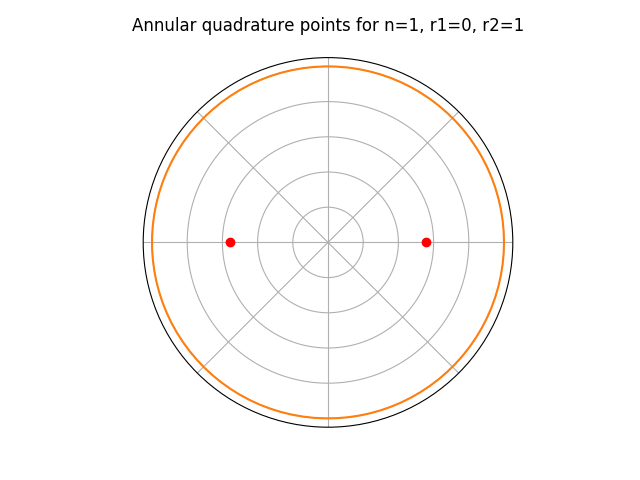
\includegraphics[scale=.5]{disk_n1}
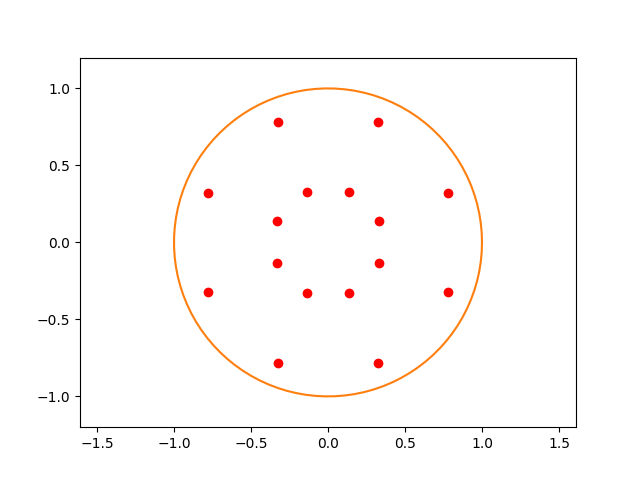
\includegraphics[scale=.5]{disk_n2}
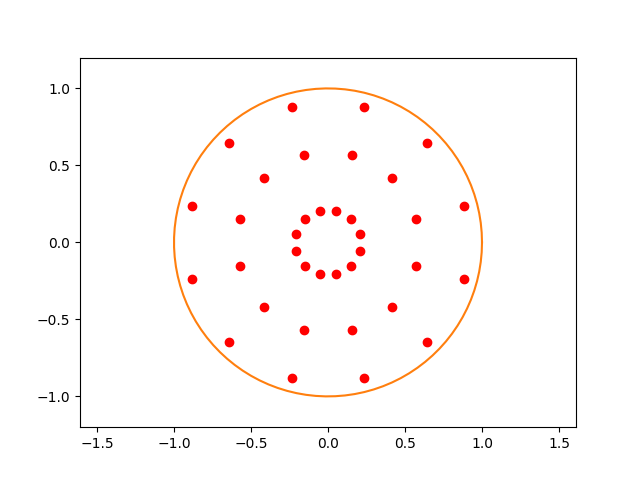
\includegraphics[scale=.5]{disk_n3}
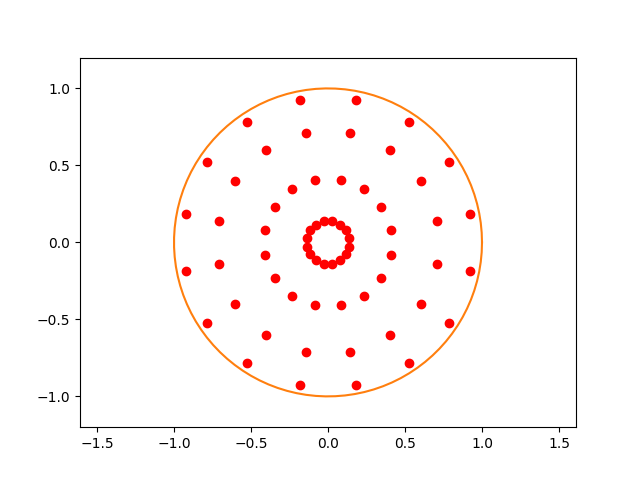
\includegraphics[scale=.5]{disk_n4}


and annulus quadrature points\\

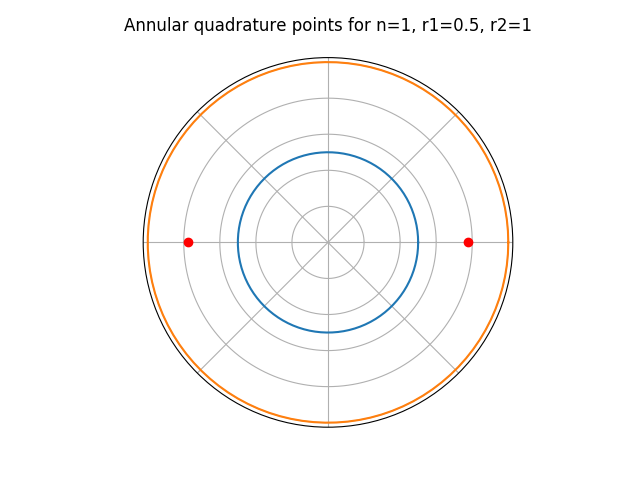
\includegraphics[scale=.5]{annulus_n1}
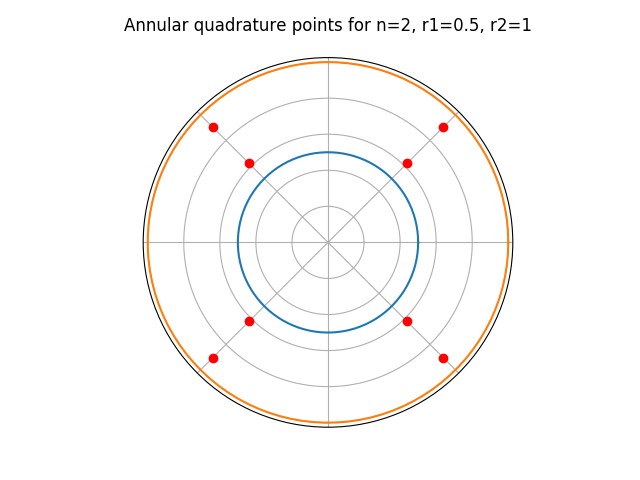
\includegraphics[scale=.5]{annulus_n2}
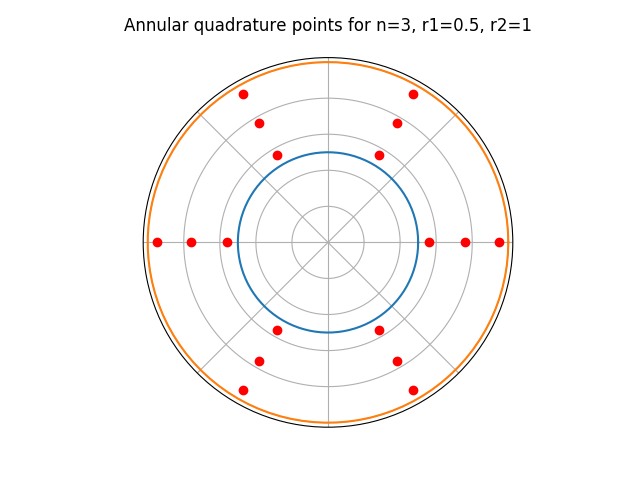
\includegraphics[scale=.5]{annulus_n3}
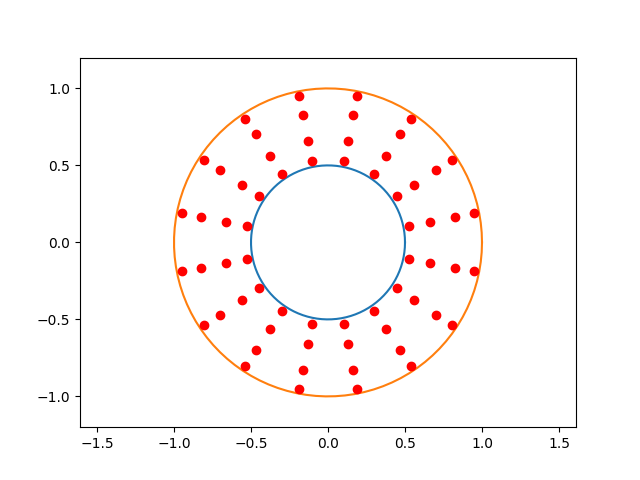
\includegraphics[scale=.5]{annulus_n4}


\end{document}